
\begin{frame}{Addresing the ITOC}

    {\huge\textbf{Third Contribution}}
    {\footnotesize
    \begin{itemize}
        \item Dynamic programming physics-informed sparse learning for closed-loop optimal control
    \end{itemize}}
    
\end{frame}

\begin{frame}{Addressing the ITOC: Trajectory Parametrization}
    \footnotesize
    \vspace*{0.02in}
    \visible<1->{Want \textbf{accurate}, \textbf{efficient}, and \textbf{generalizable} on-board solutions to \textbf{non-linear OCPs},}
    \begin{columns}
        \begin{column}{0.7\textwidth}
            \only<1>{
                \begin{figure}
                    \centering
                    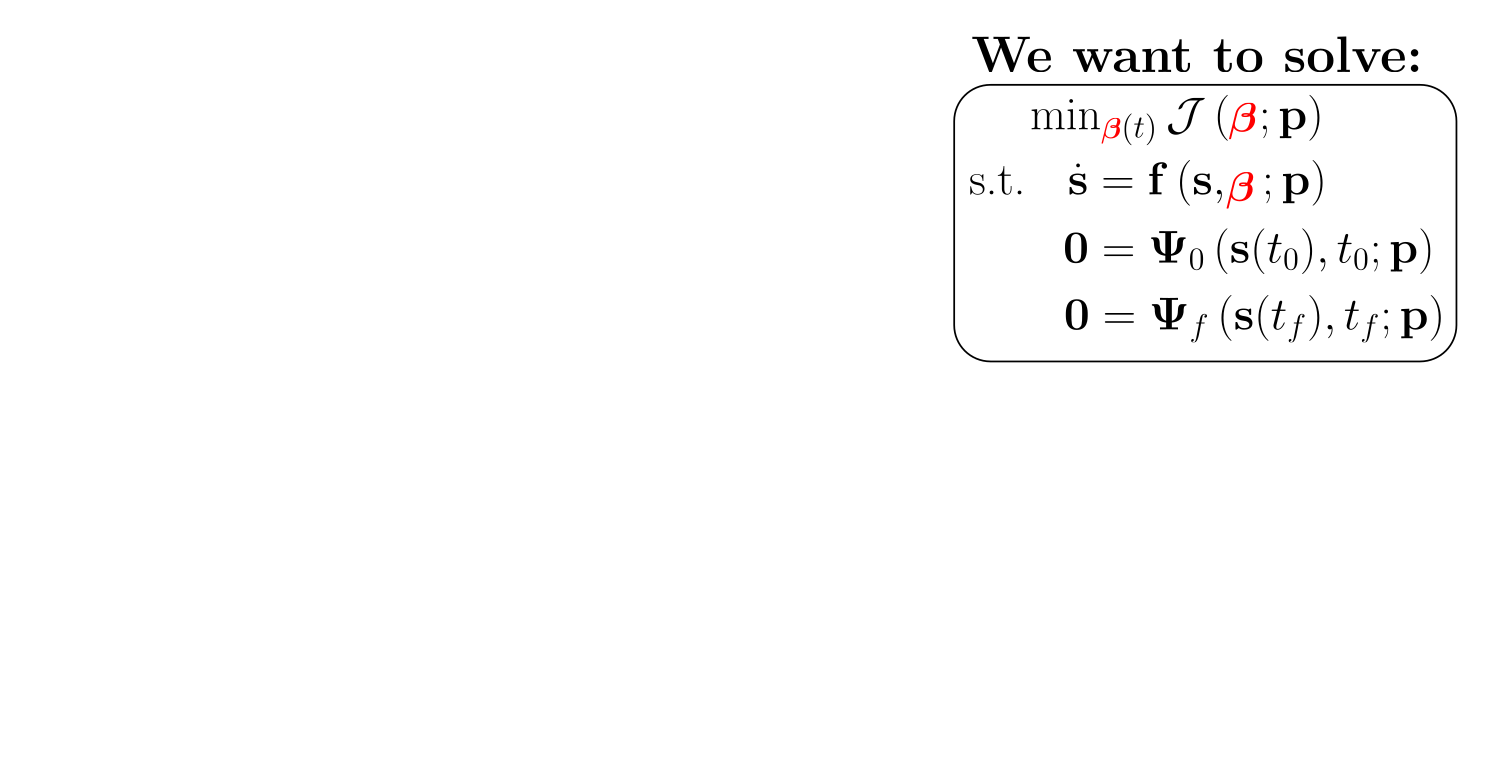
\includegraphics[width=0.9\textwidth]{../figs/sparsehjb/trajectory_parametrization_1.png}
                \end{figure}}
            \only<2>{
                \begin{figure}
                    \centering
                    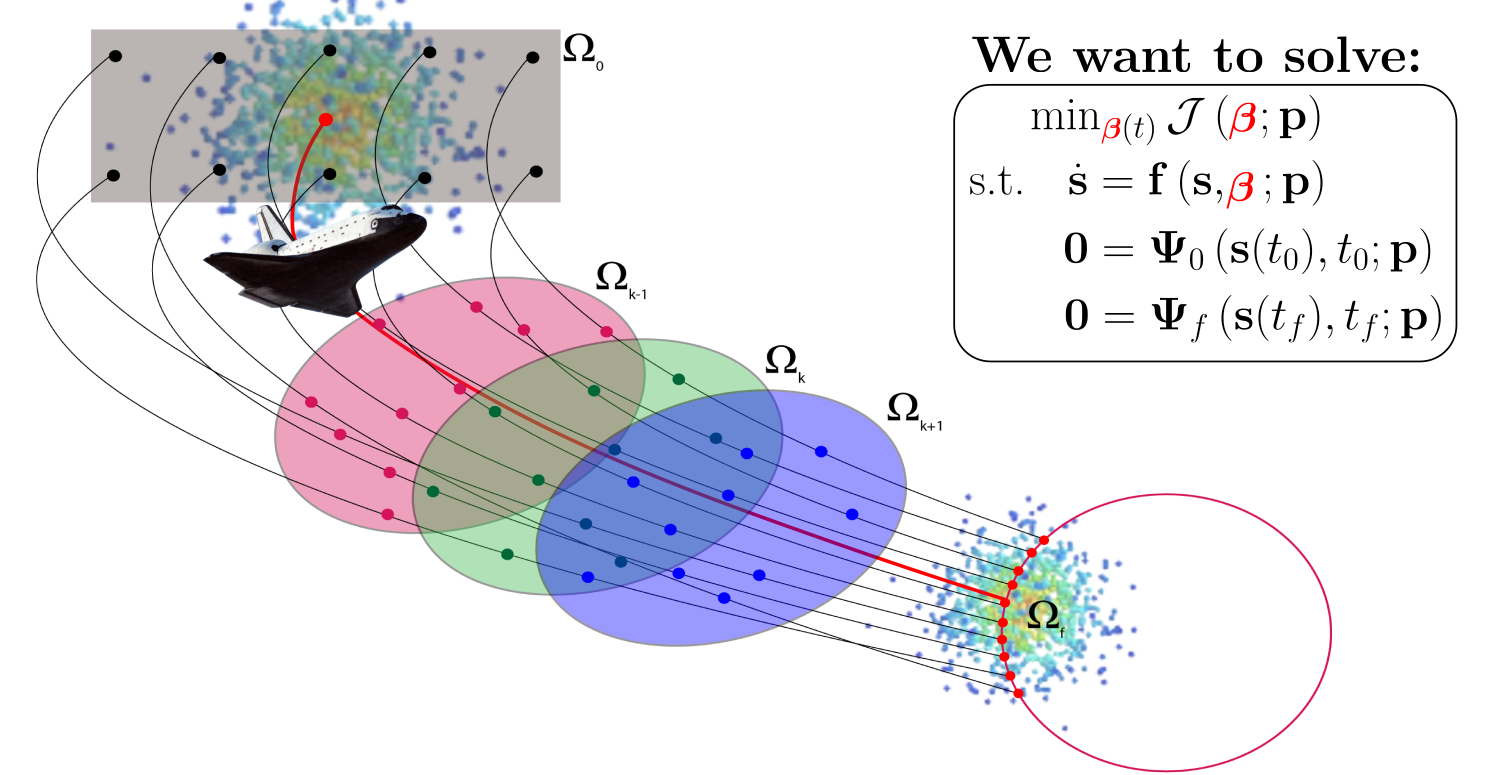
\includegraphics[width=0.9\textwidth]{../figs/sparsehjb/trajectory_parametrization_2.png}
                \end{figure}}
            \only<3->{
                \begin{figure}
                    \centering
                    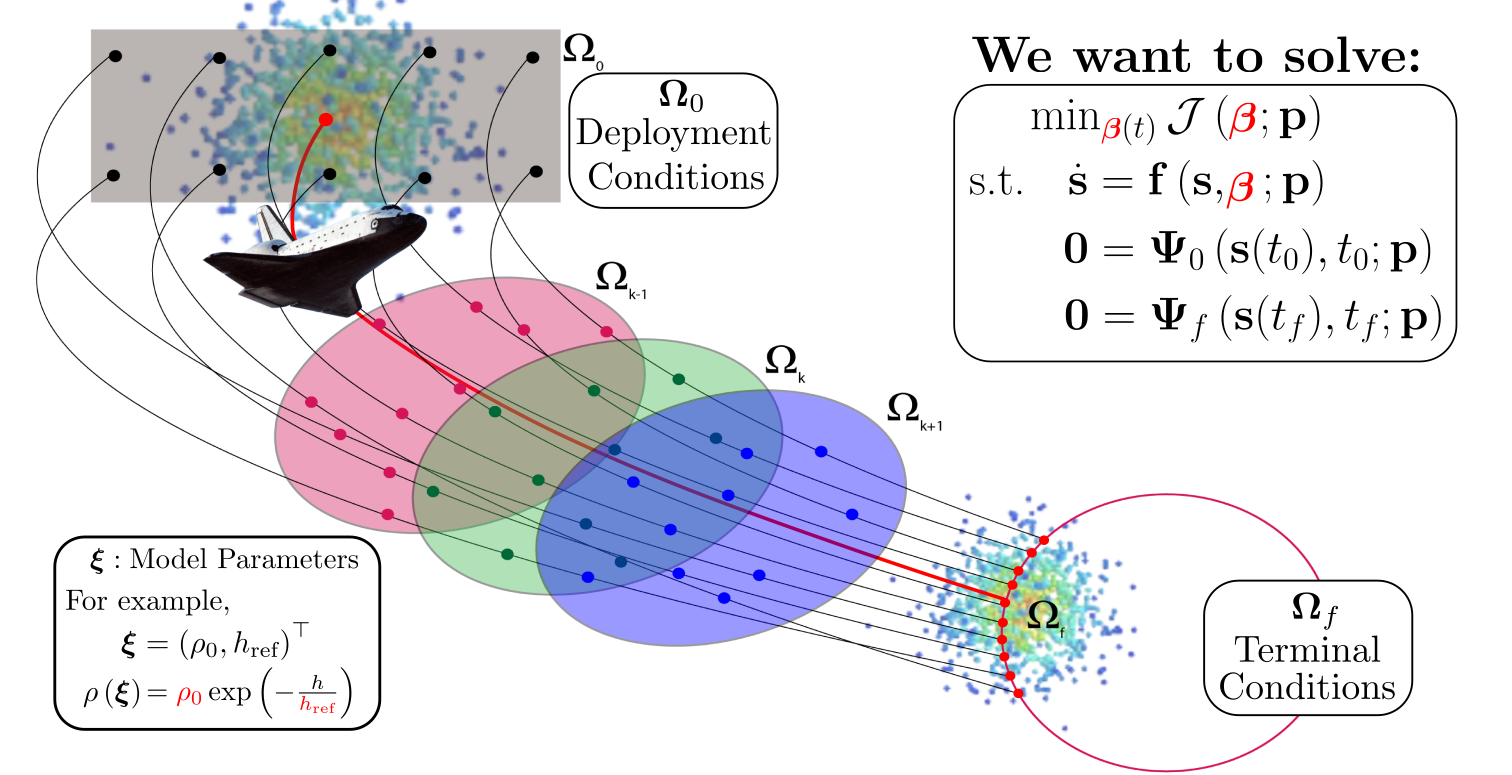
\includegraphics[width=0.9\textwidth]{../figs/sparsehjb/trajectory_parametrization_3.png}
                \end{figure}}
        \end{column}
        \hspace*{-0.2in}
        \begin{column}{0.4\textwidth}
            \visible<4->{
            \begin{graybox}{Parametrization}
                \visible<5->{
                Parameters,
                \vspace*{-0.05in}
                \begin{equation*}
                    \vp = \left(\vOmega_0,\vOmega_f,\vxi\right)^\top\in\mathbb{R}^{n_p}
                \end{equation*}}
                \visible<6->{
                are, e.g., normally distributed,
                \vspace*{-0.05in}
                \begin{equation*}
                    \vp\sim\mathcal{N}\left(\mathbf{m},\boldsymbol{\sigma}\right)
                \end{equation*}}
                \visible<7->{
                where,
                \vspace*{-0.05in}
                \begin{itemize}
                    \item $\mathbf{m}$: nominal mission,
                    \item $\boldsymbol{\sigma}$: mission uncertainty
                \end{itemize}}
            \end{graybox}}
        \end{column}
    \end{columns}
\end{frame}

\begin{frame}{Addressing the ITOC: New Formulation}
    \footnotesize
    \visible<1->{Generate a \textbf{distribution of optimal paths} as a function of $\vp$},
    \vspace*{-0.1in}
    \only<1>{
        \begin{figure}
            \centering
            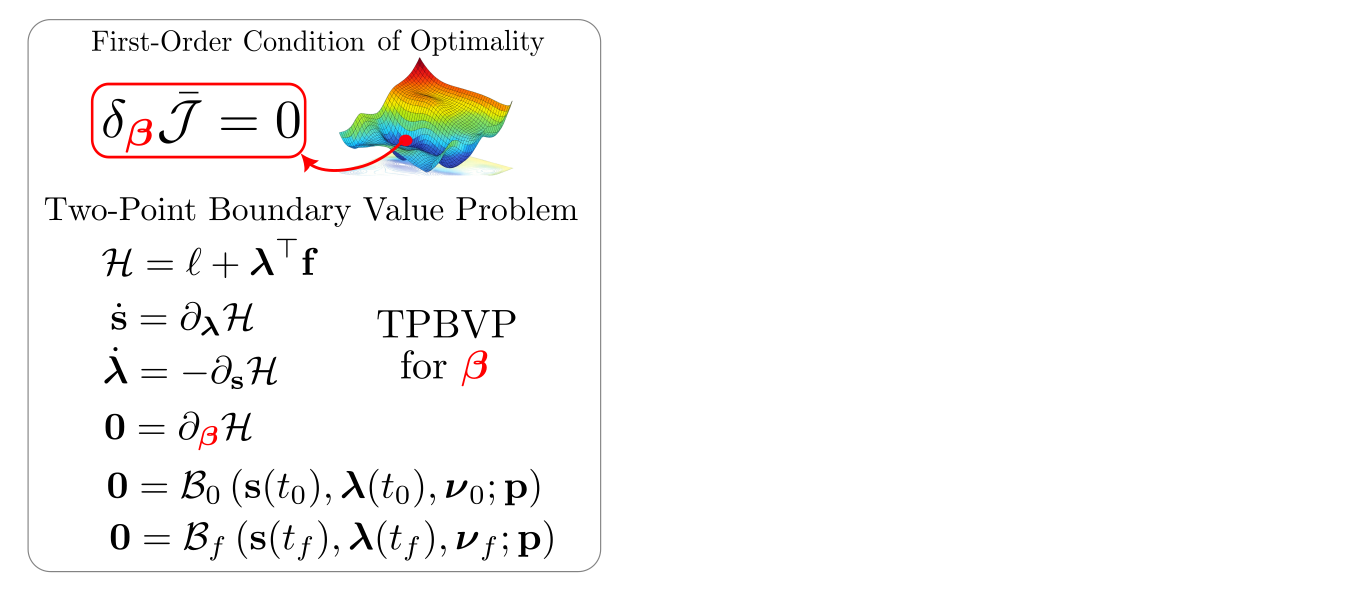
\includegraphics[width=0.9\textwidth]{../figs/sparsehjb/solutions_1.png}
        \end{figure}}
    \only<2>{
        \begin{figure}
            \centering
            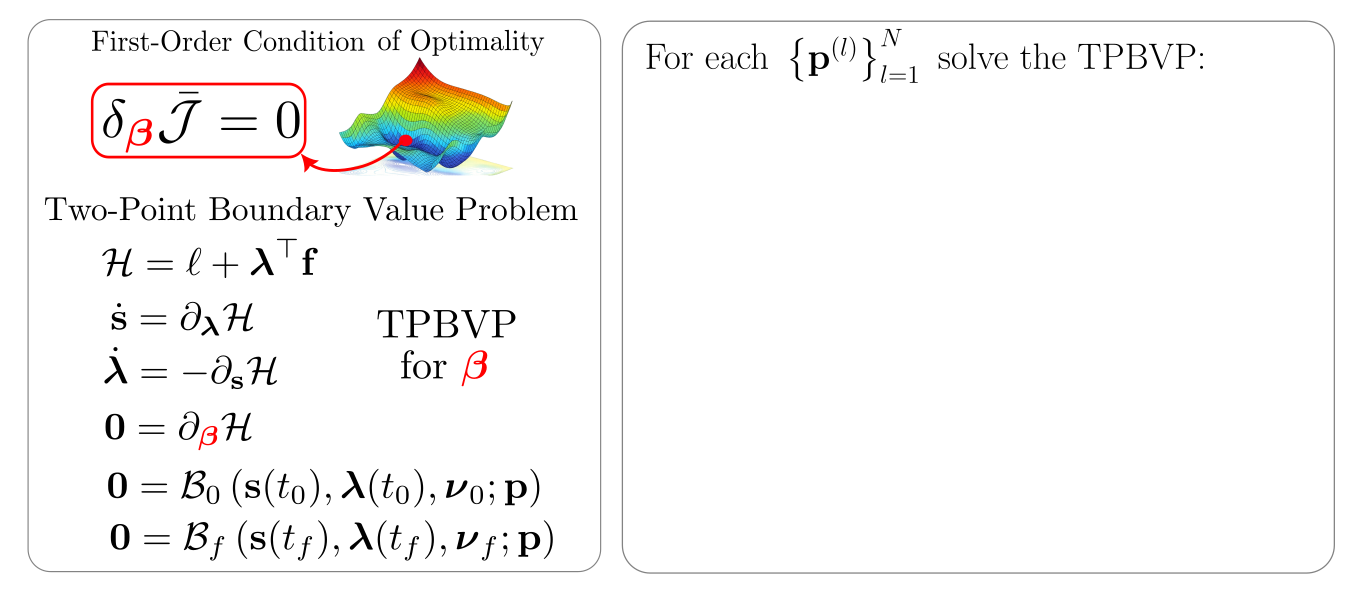
\includegraphics[width=0.9\textwidth]{../figs/sparsehjb/solutions_2.png}
        \end{figure}}
    \only<3>{
        \begin{figure}
            \centering
            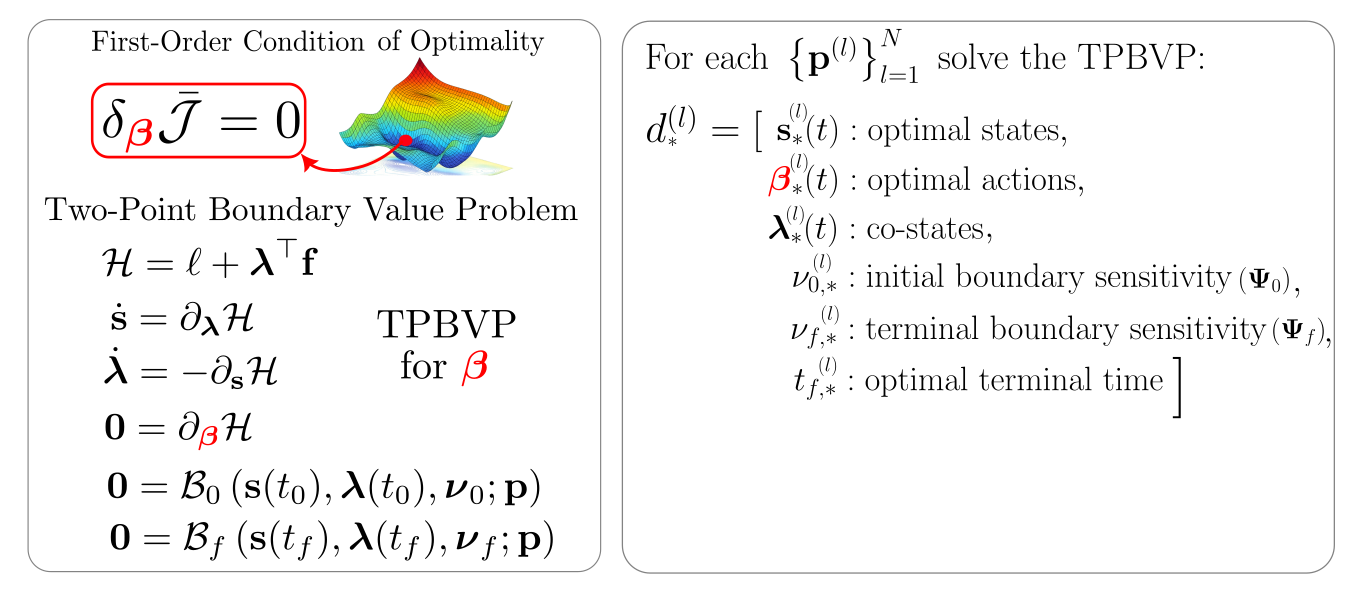
\includegraphics[width=0.9\textwidth]{../figs/sparsehjb/solutions_3.png}
        \end{figure}}
    \only<4>{
        \begin{figure}
            \centering
            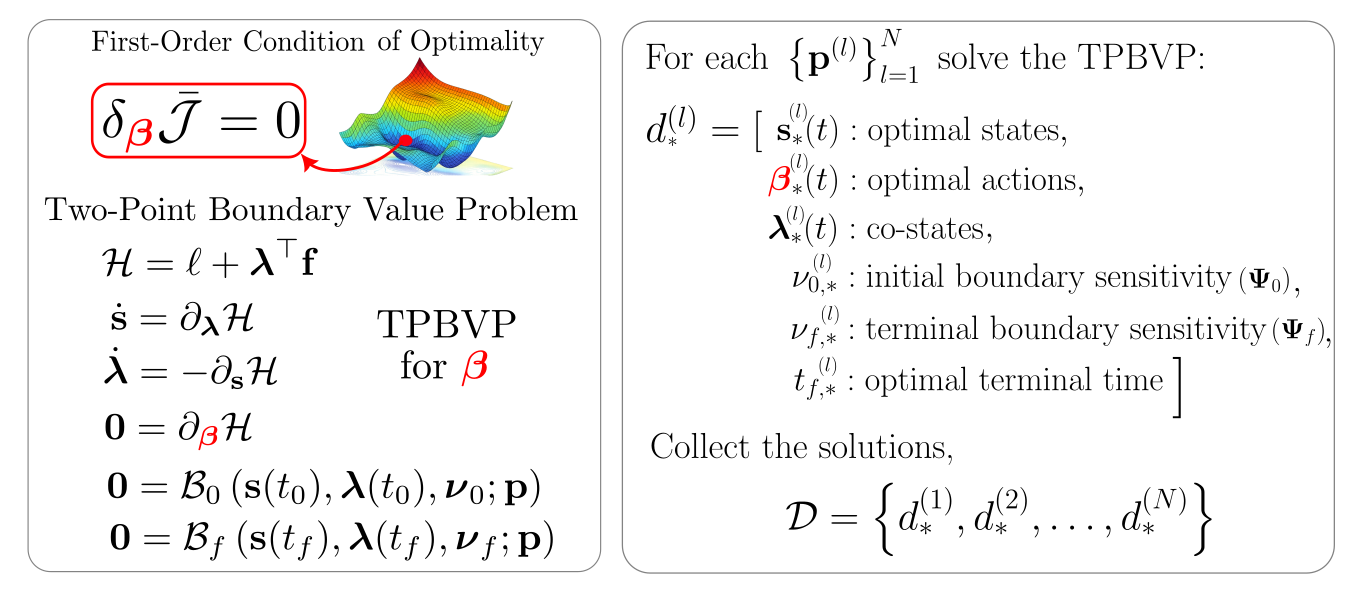
\includegraphics[width=0.9\textwidth]{../figs/sparsehjb/solutions_4.png}
        \end{figure}}
\end{frame}

\begin{frame}{Addressing the ITOC: New Formulation}
    \footnotesize
    \visible<1->{Learn the value function from the \textbf{distribution of optimal paths},}
    \only<2>{
        \begin{figure}
            \centering
            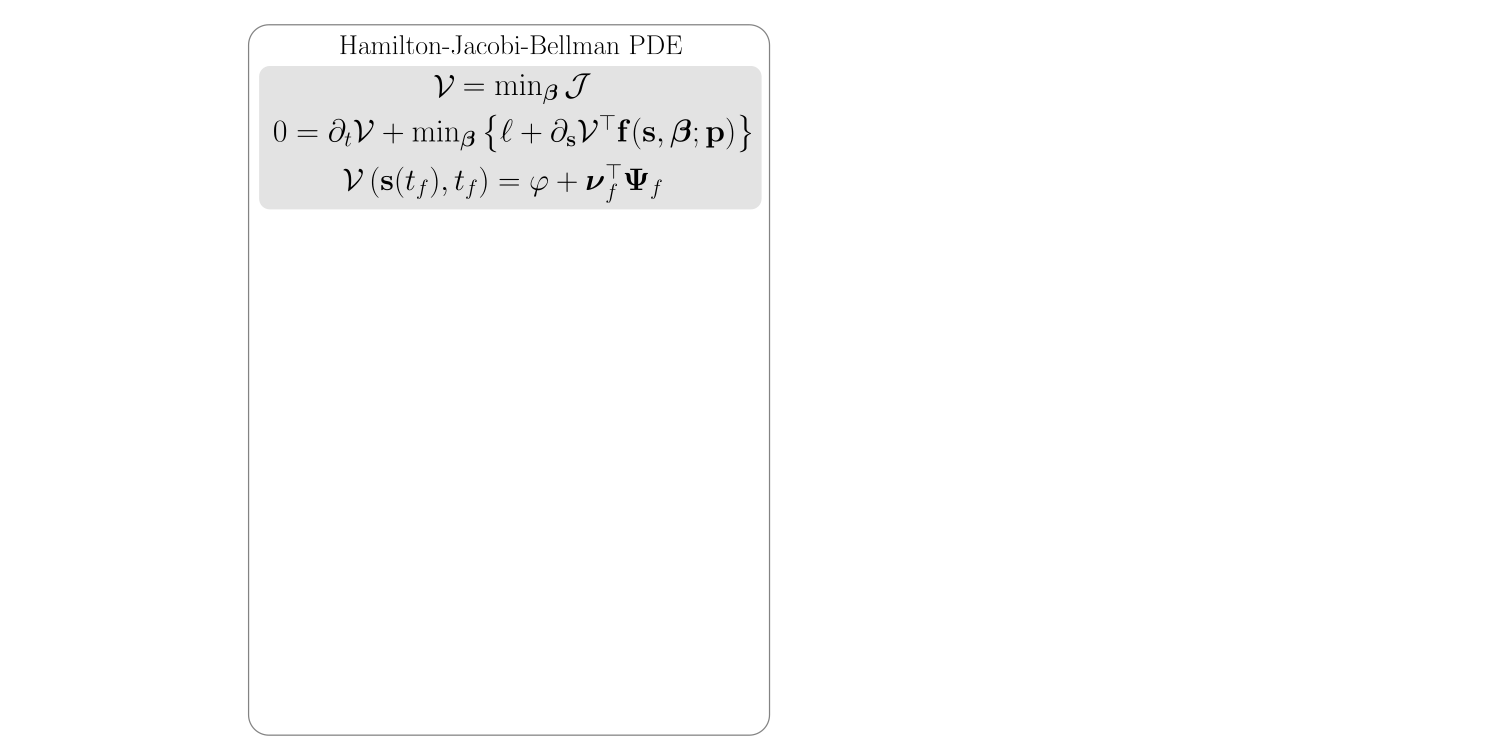
\includegraphics[width=0.95\textwidth]{../figs/sparsehjb/characteristics_1.png}
        \end{figure}}
    \only<3>{
        \begin{figure}
            \centering
            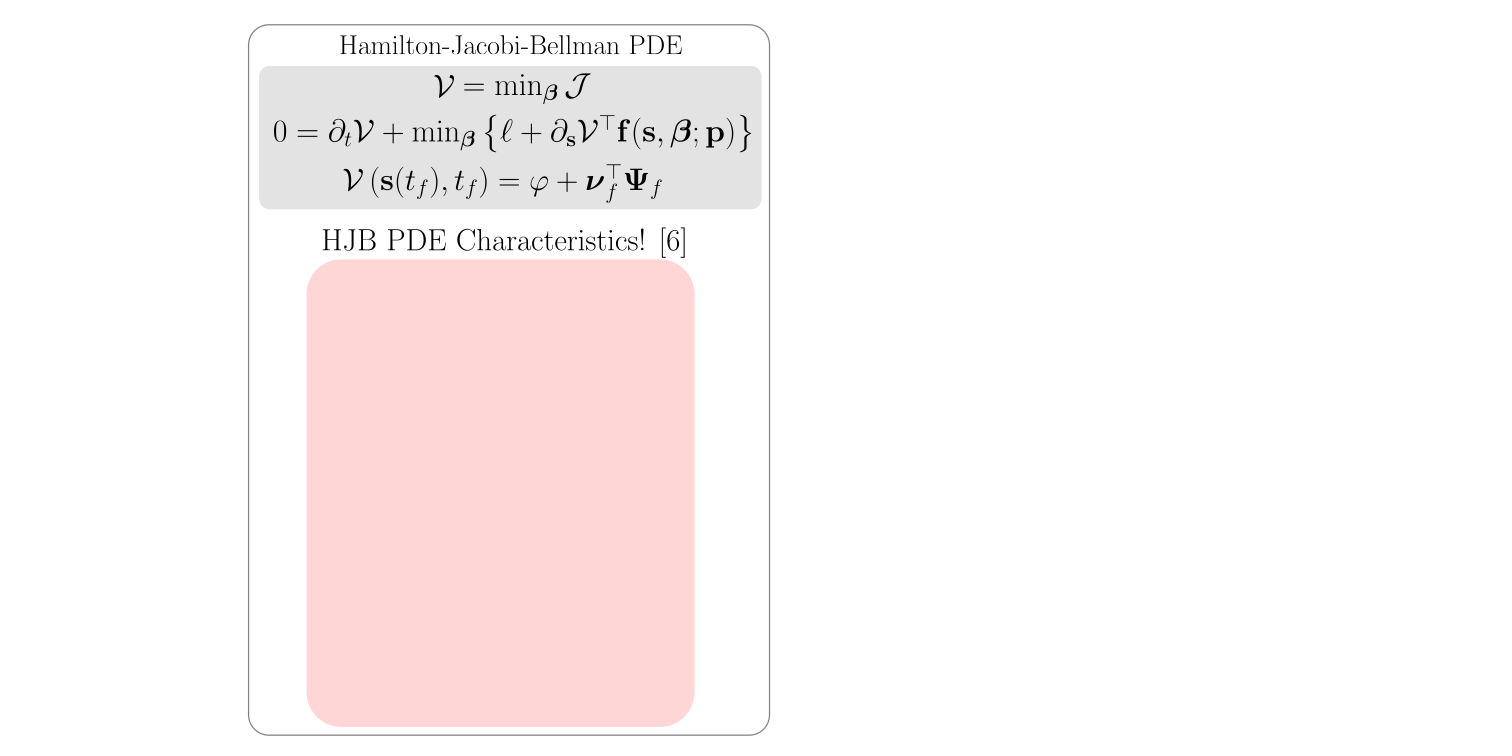
\includegraphics[width=0.95\textwidth]{../figs/sparsehjb/characteristics_2.png}
        \end{figure}}
    \only<4>{
        \begin{figure}
            \centering
            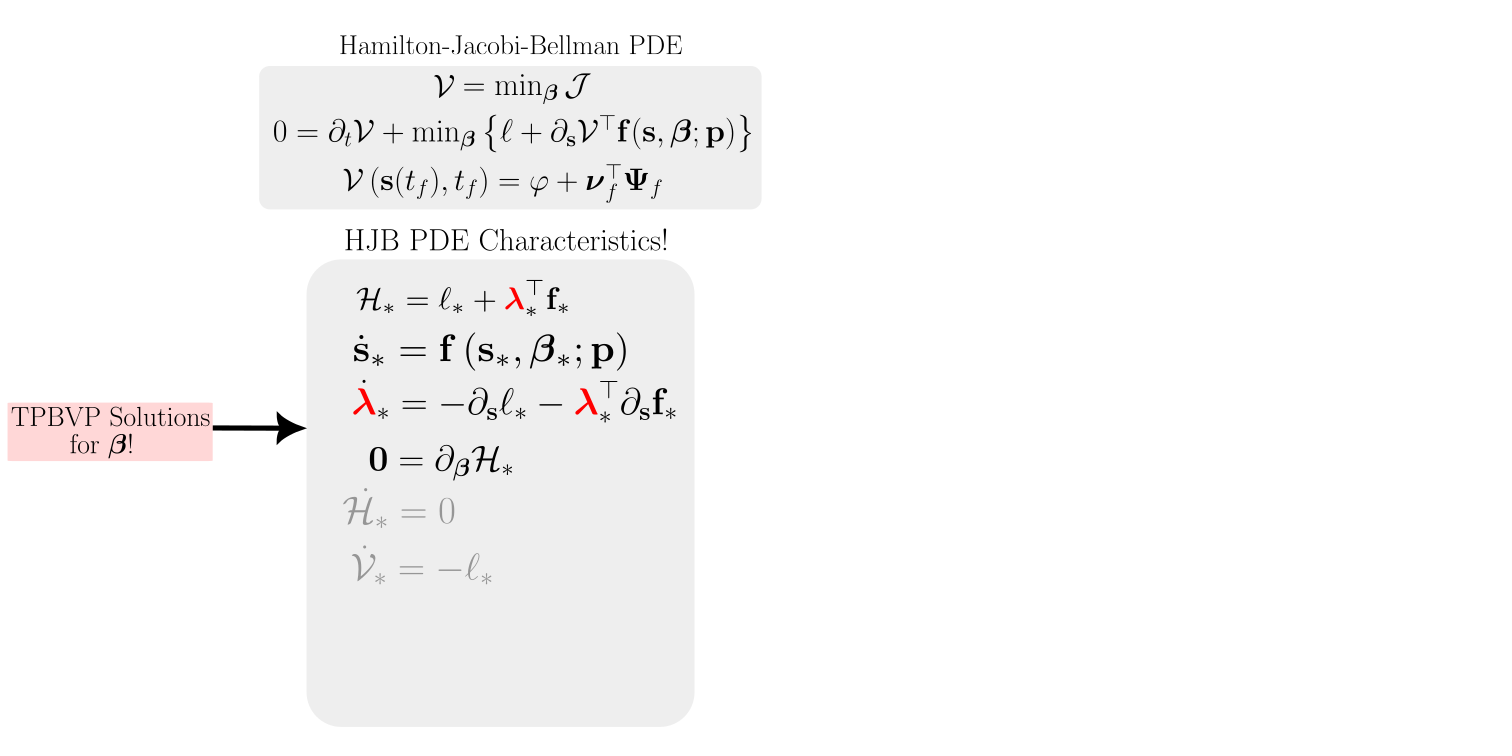
\includegraphics[width=0.95\textwidth]{../figs/sparsehjb/characteristics_3.png}
        \end{figure}}
    \only<5>{
        \begin{figure}
            \centering
            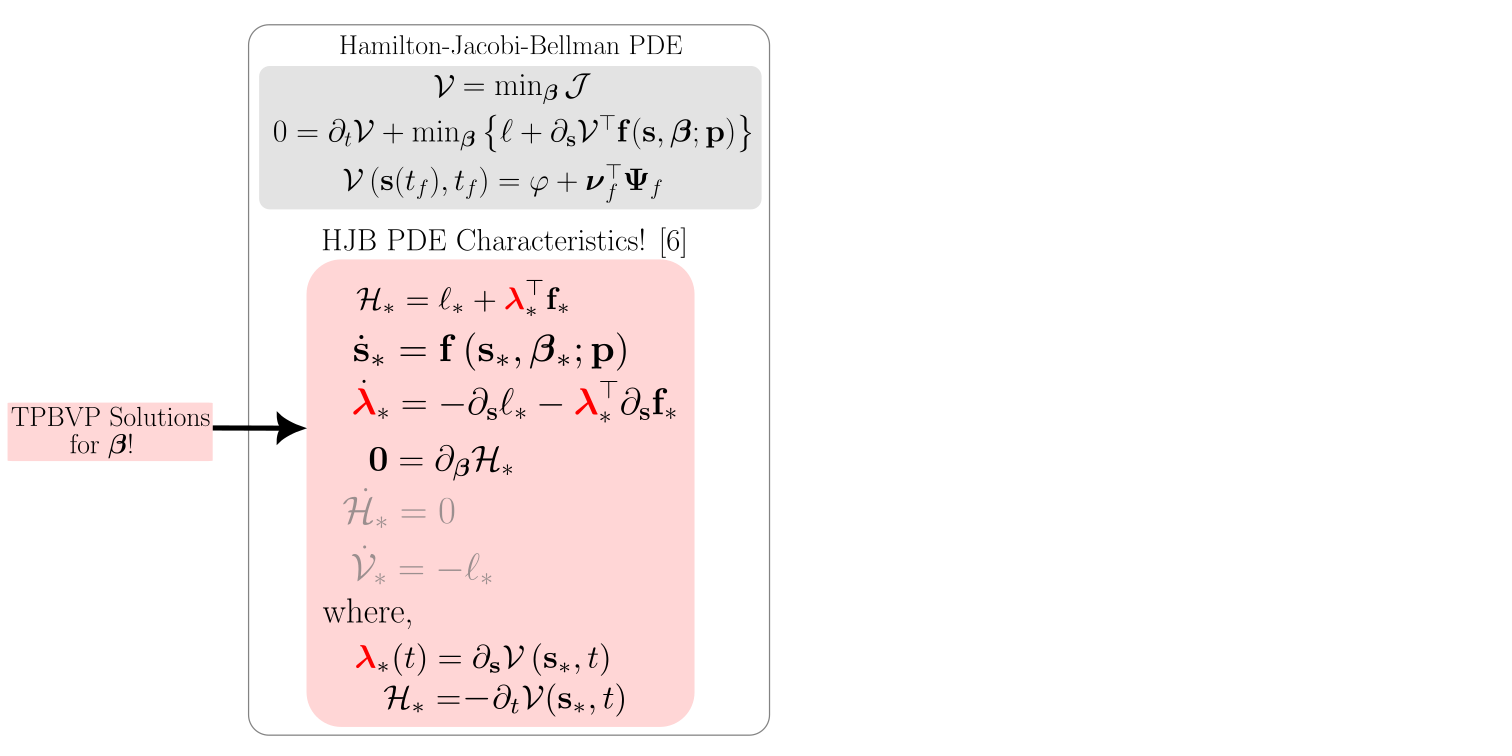
\includegraphics[width=0.95\textwidth]{../figs/sparsehjb/characteristics_4.png}
        \end{figure}}
    \only<6>{
        \begin{figure}
            \centering
            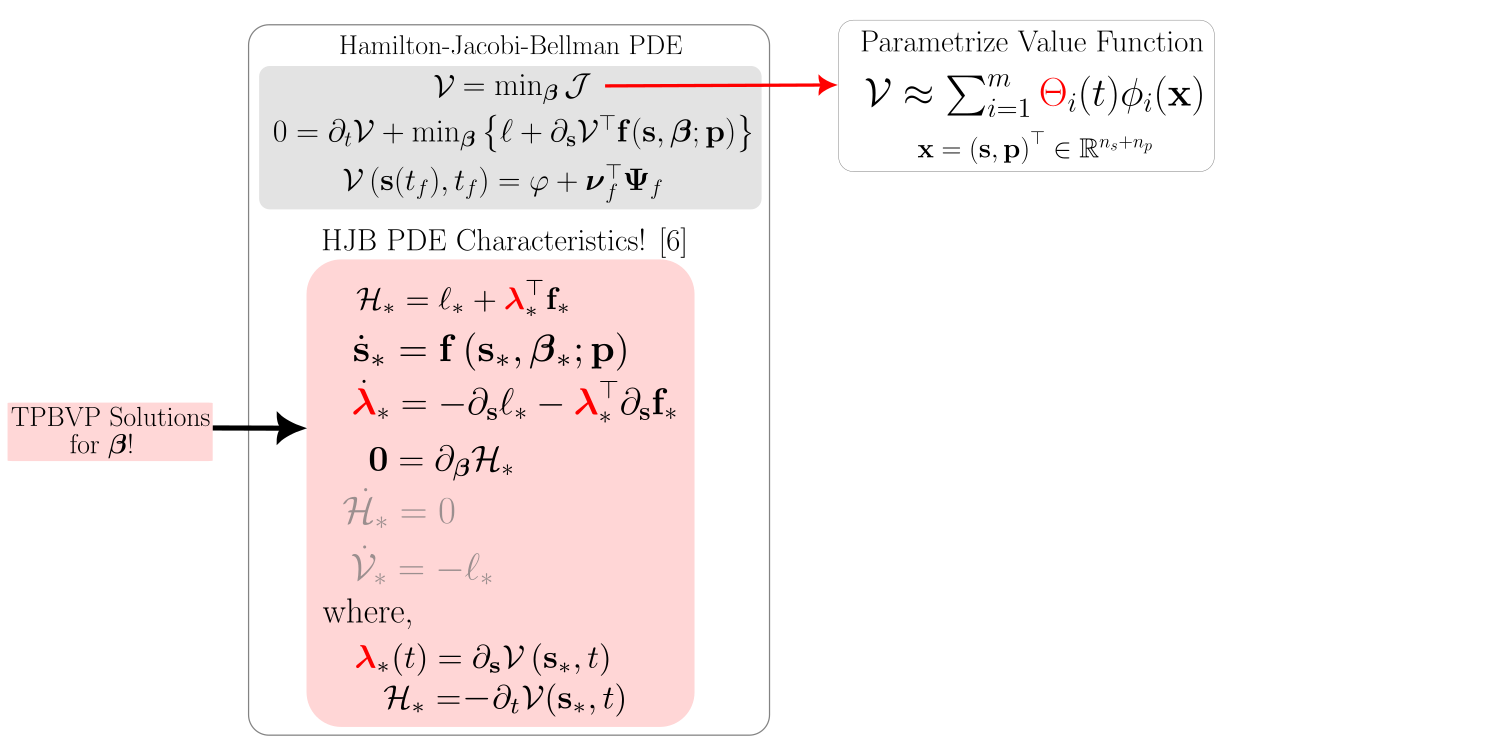
\includegraphics[width=0.95\textwidth]{../figs/sparsehjb/characteristics_5.png}
        \end{figure}}
    \only<7>{
        \begin{figure}
            \centering
            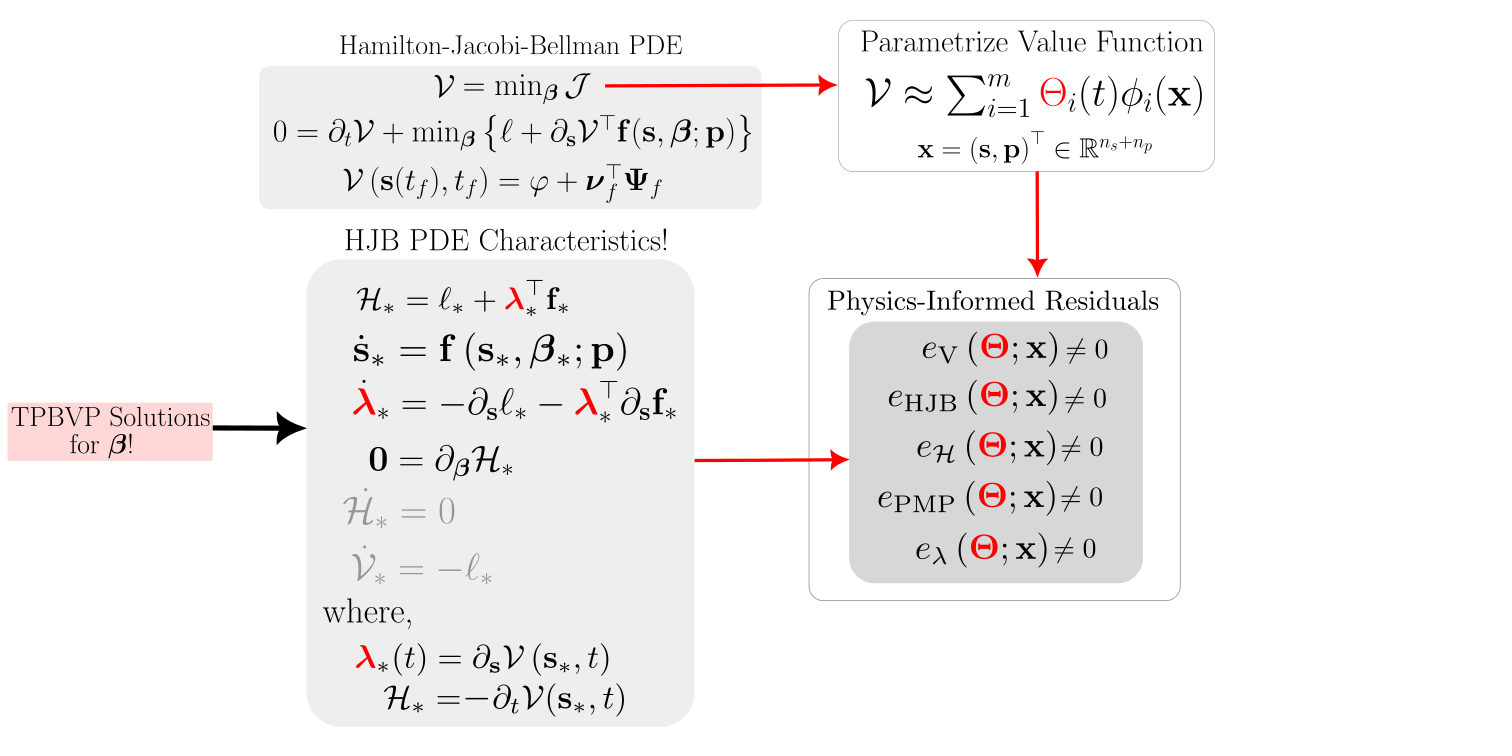
\includegraphics[width=0.95\textwidth]{../figs/sparsehjb/characteristics_6.png}
        \end{figure}}
    \only<8>{
        \begin{figure}
            \centering
            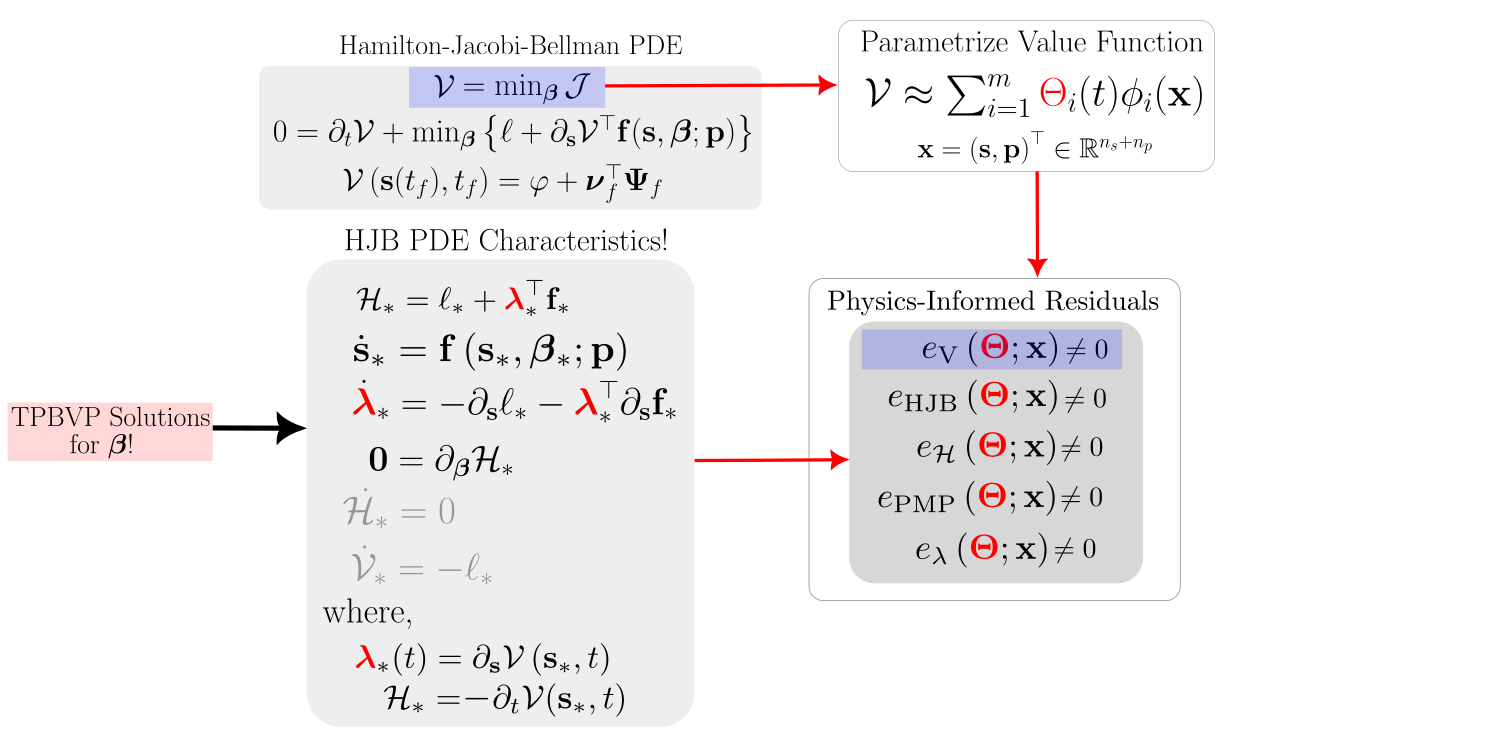
\includegraphics[width=0.95\textwidth]{../figs/sparsehjb/characteristics_7.png}
        \end{figure}}
    \only<9>{
        \begin{figure}
            \centering
            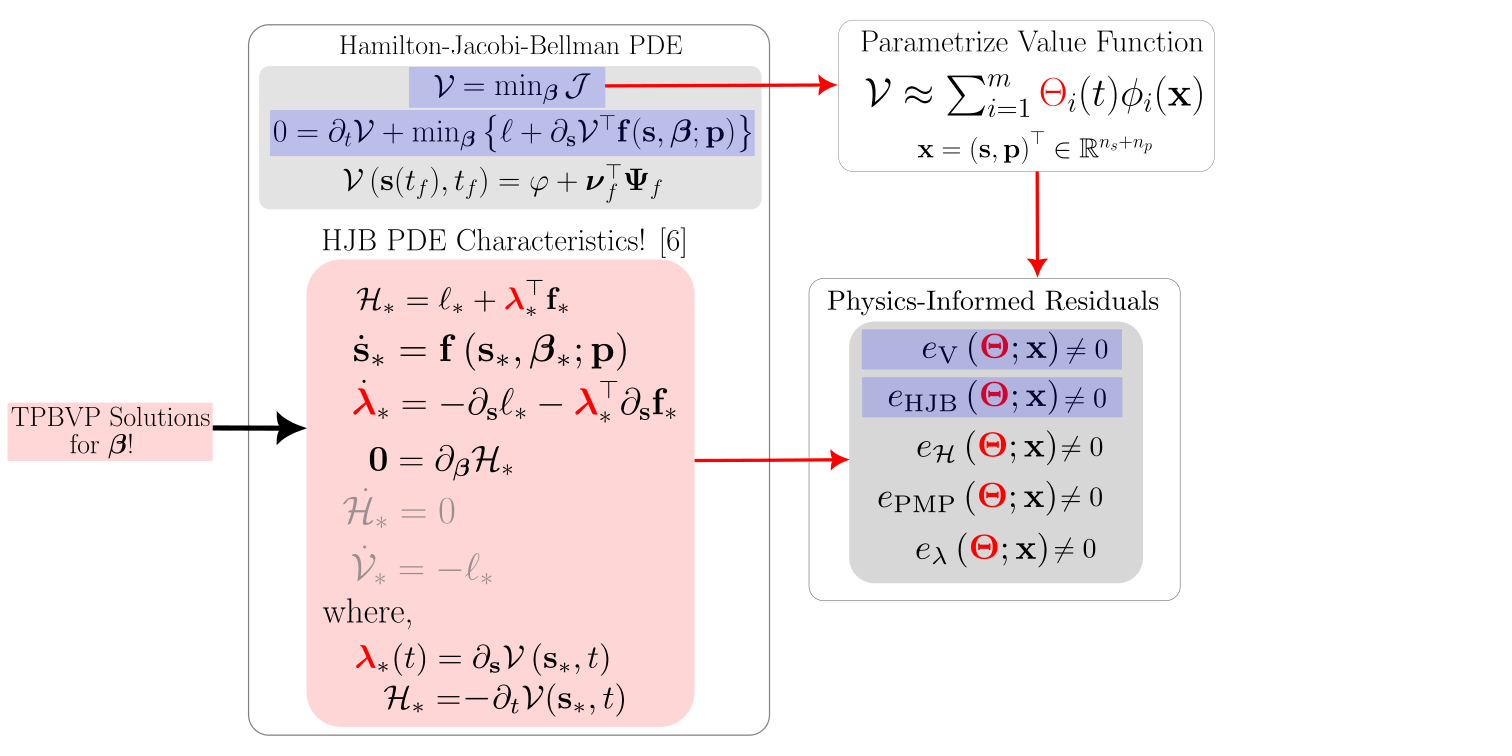
\includegraphics[width=0.95\textwidth]{../figs/sparsehjb/characteristics_8.png}
        \end{figure}}
    \only<10>{
        \begin{figure}
            \centering
            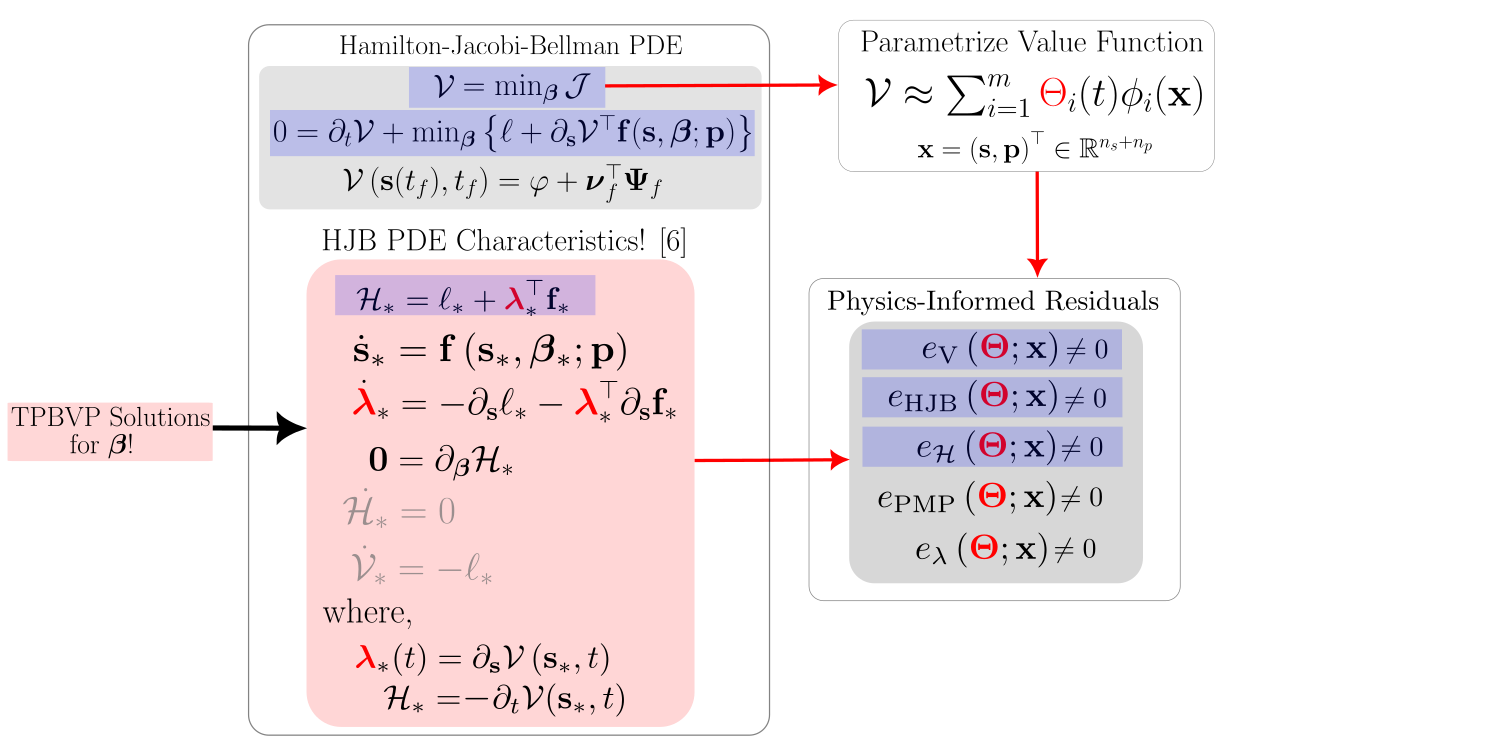
\includegraphics[width=0.95\textwidth]{../figs/sparsehjb/characteristics_9.png}
        \end{figure}}
    \only<11>{
        \begin{figure}
            \centering
            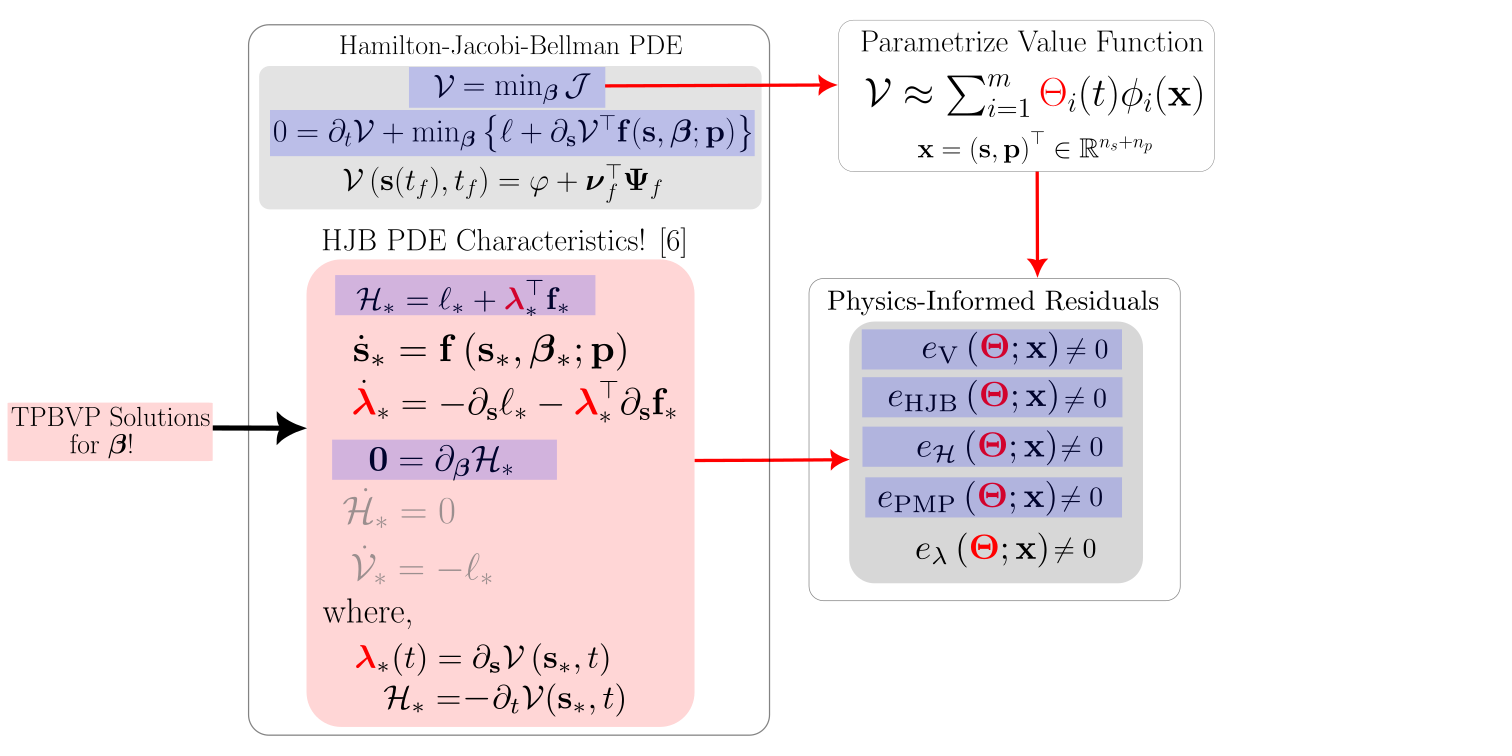
\includegraphics[width=0.95\textwidth]{../figs/sparsehjb/characteristics_10.png}
        \end{figure}}
    \only<12>{
        \begin{figure}
            \centering
            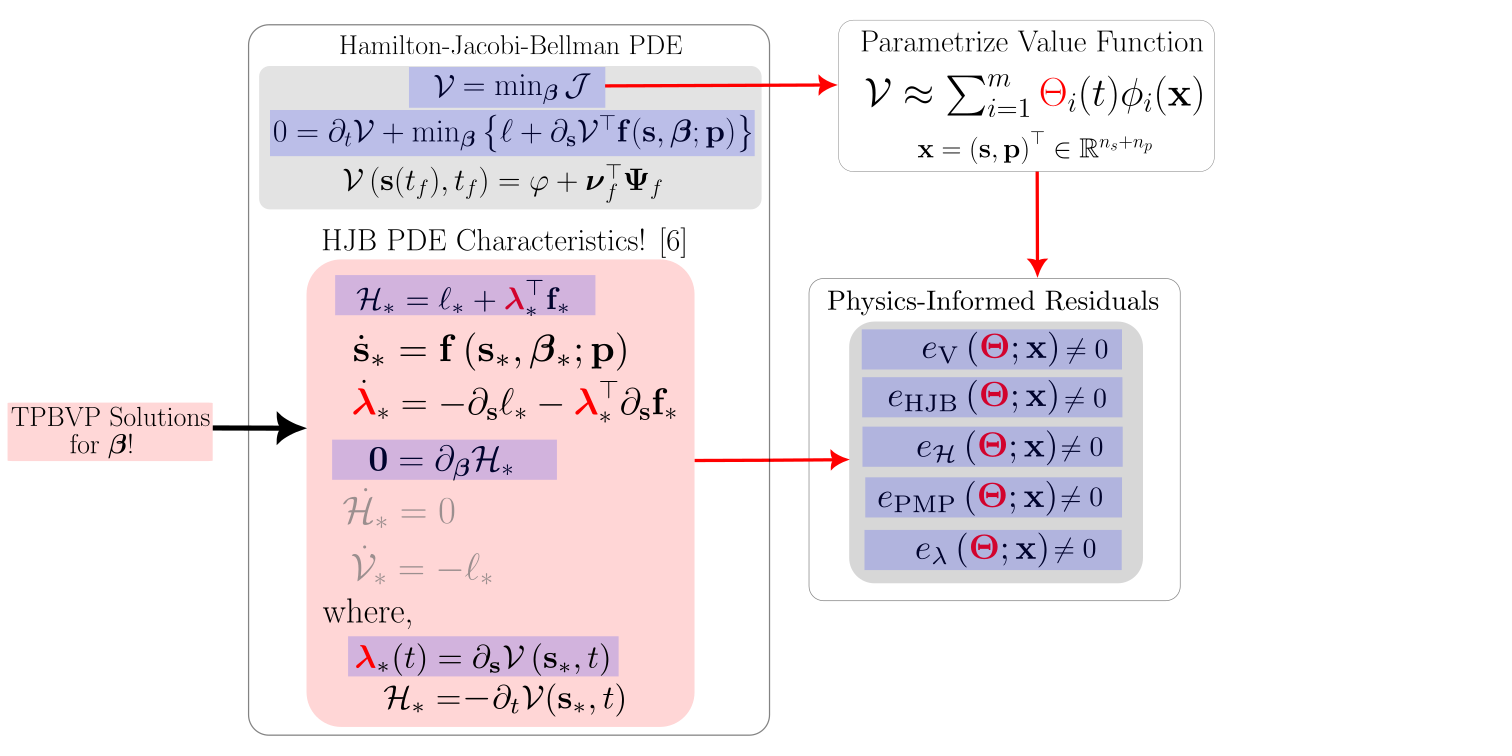
\includegraphics[width=0.95\textwidth]{../figs/sparsehjb/characteristics_11.png}
        \end{figure}}
    \only<13>{
        \begin{figure}
            \centering
            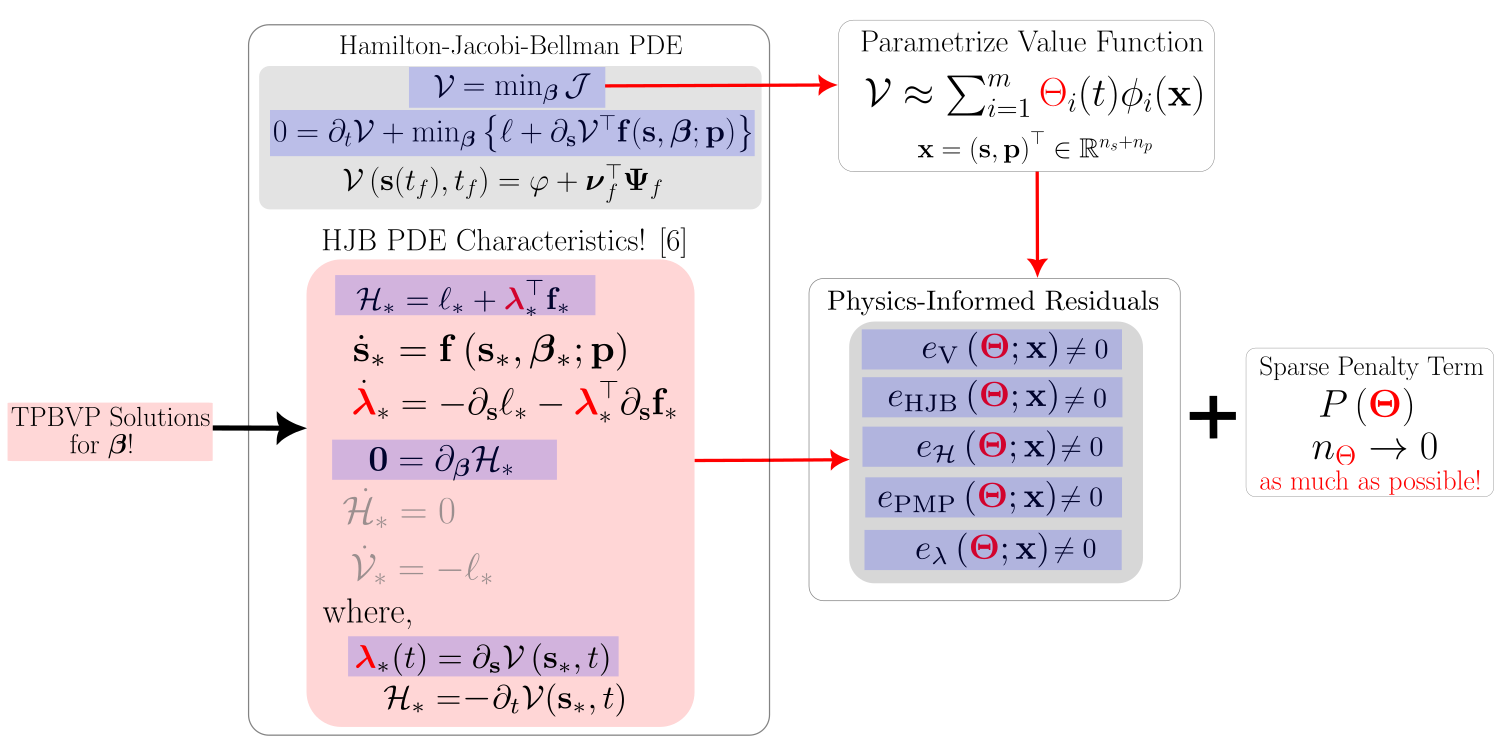
\includegraphics[width=0.95\textwidth]{../figs/sparsehjb/characteristics_12.png}
        \end{figure}}
\end{frame}